% 
% 
%			5: Market-basket
\chapter{Market-basket analysis}
\label{chap:market-basket}

Now when the frequent pairs are defined, the corresponding association rules can be determined.
The \texttt{support} metric of the association rule alone can be misleading: for example, the support of the association rule of two independently popular items might be high, but such rules are useless from marketing point of view. 
\texttt{confidence} and \texttt{interest} metrics can help us gain more valuable insights.
\begin{itemize}
	\item \texttt{confidence} of the association rule - is the fraction of the baskets with all of \textit{I} that also contain \textit{j};
	\item \texttt{interest} of the rule -is the difference between its confidence and the fraction of baskets that contain \textit{j}.
\end{itemize}

The cosine similarity was used to determine the same books with slightly different titles to clear the resulting association rules. 
By controlling the metrics of the association-rules some interesting and useful rules can be found.

\begin{figure}[h]
	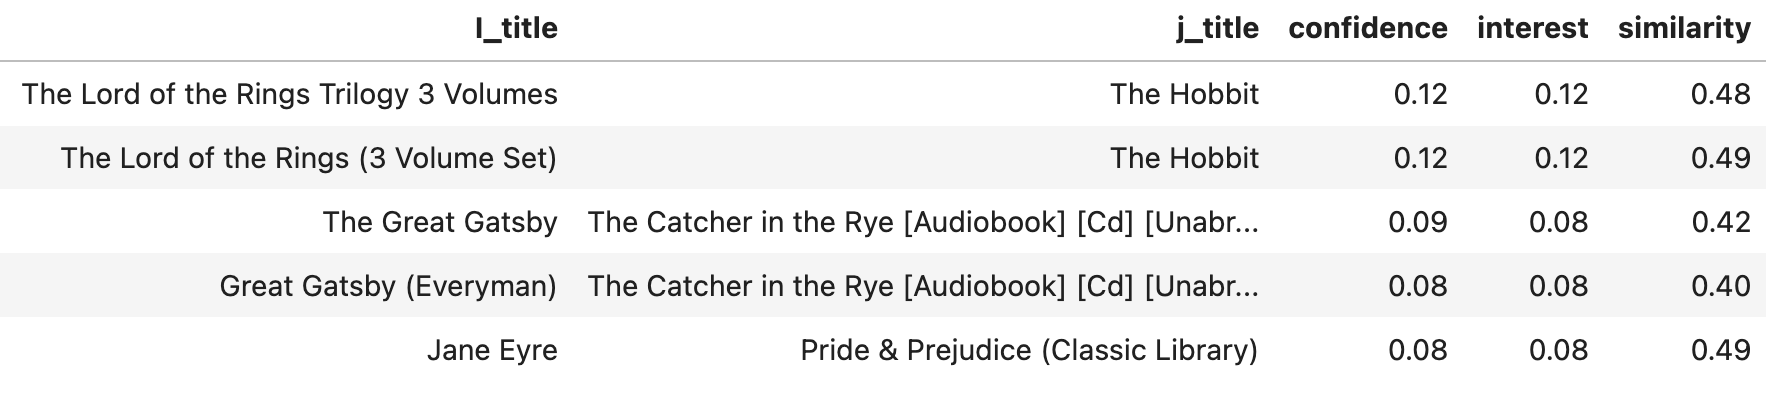
\includegraphics[width=14cm]{images/5-association_rules}
\centering
\end{figure}

\newpage
The association rule can be represented by a network chart.

\begin{figure}[h]
	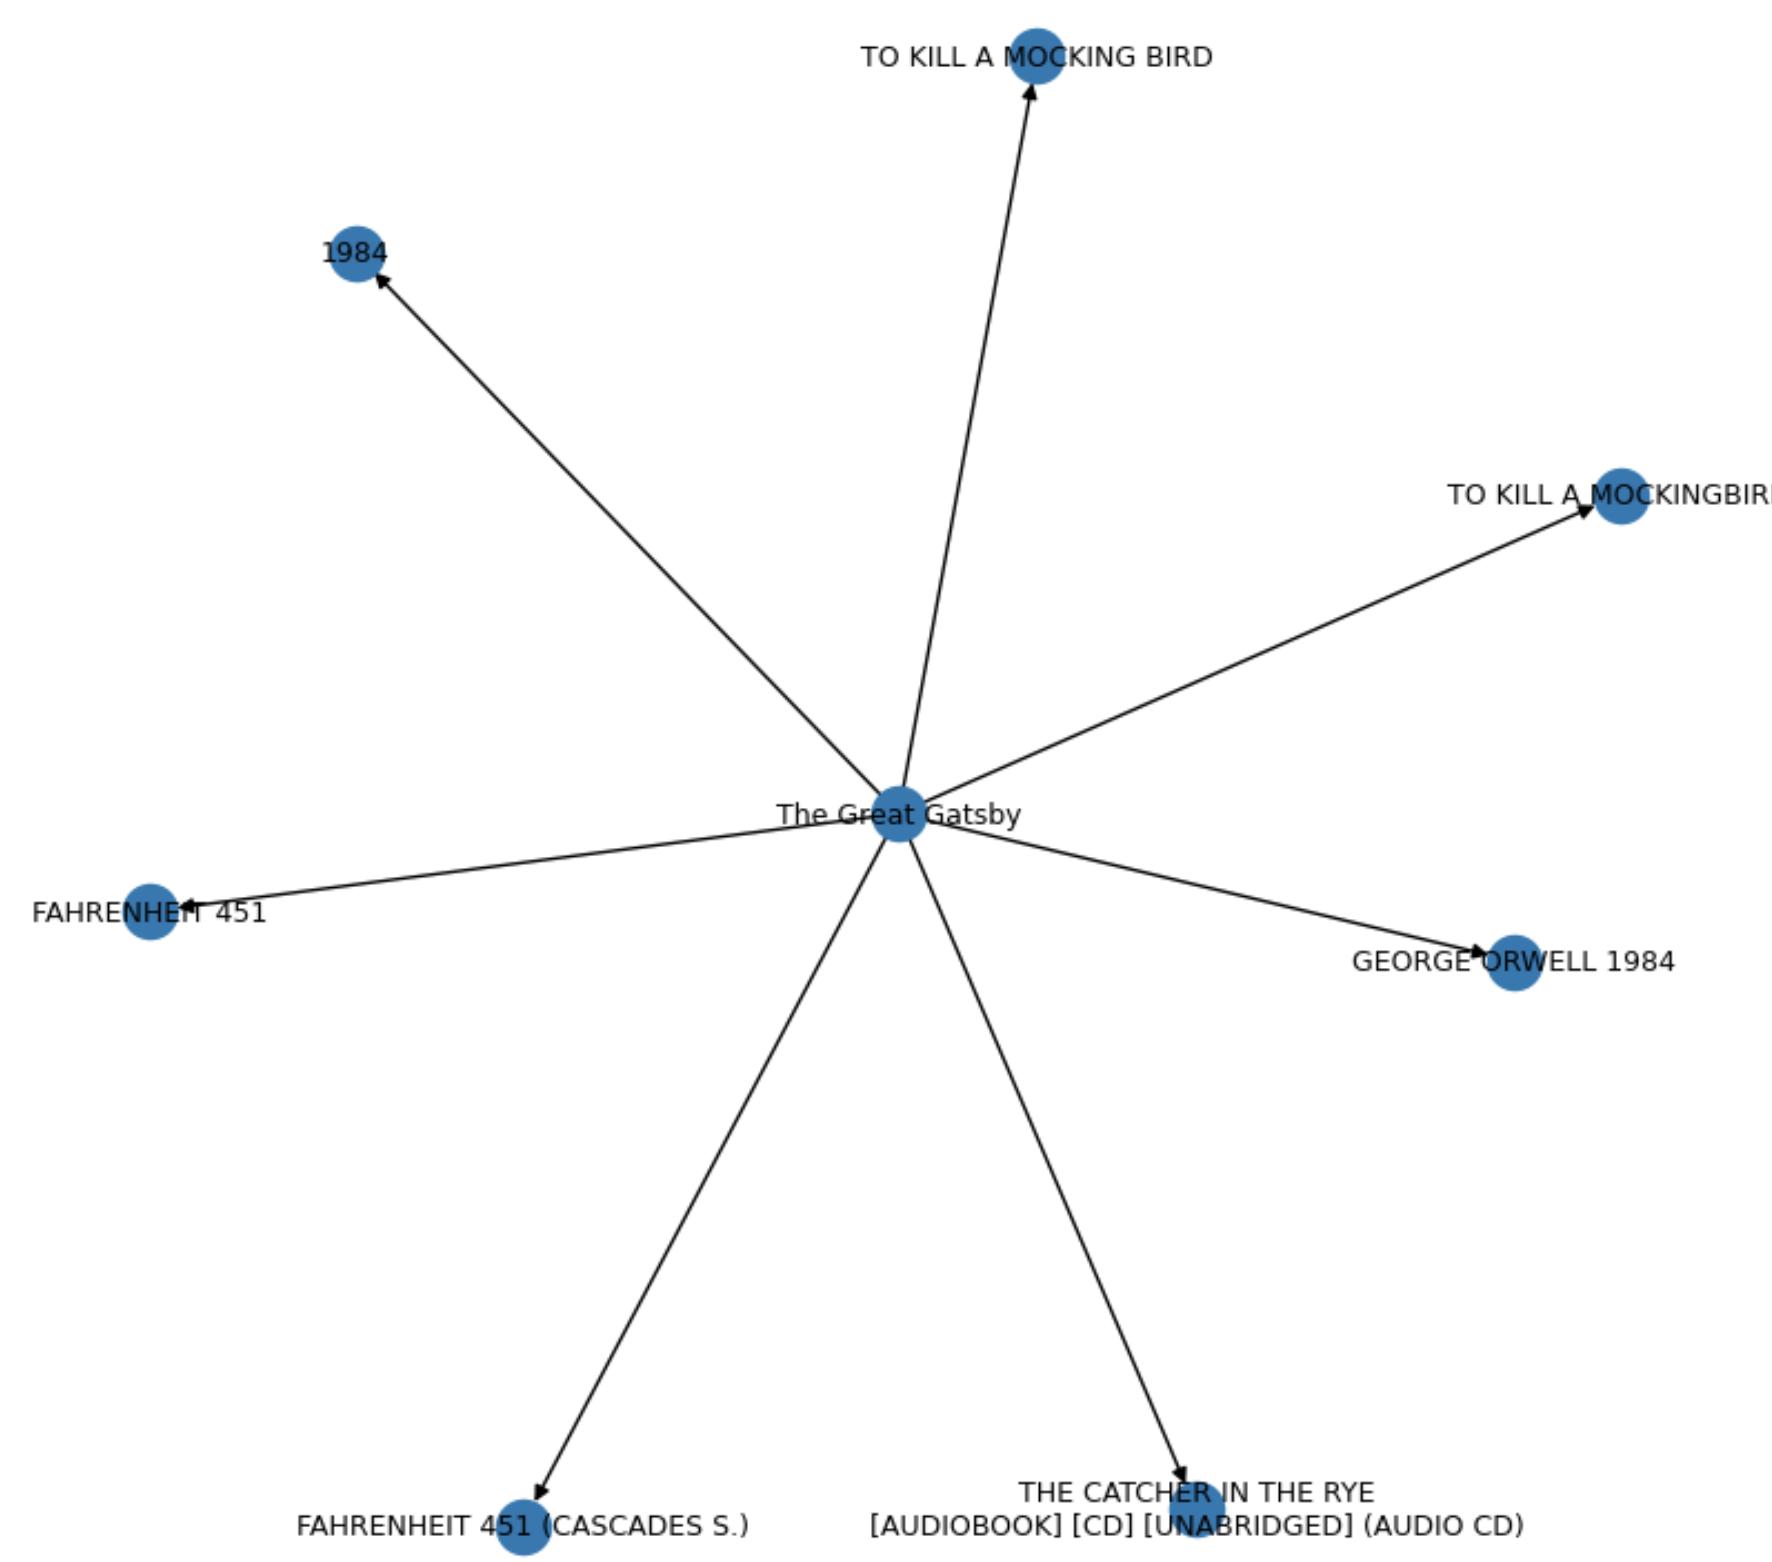
\includegraphics[width=12cm]{images/5-gatsby_associations}
\centering
\end{figure}


